\documentclass{paper}
\usepackage{xeCJK}
\usepackage{listings}
\usepackage{hyperref}
\usepackage{amsmath,amssymb,amsthm}
\usepackage{xcolor}

%\lstset
%{
%    basicstyle=\ttfamily,
%    numbers=left,
%    % numberstyle=\tiny,
%    keywordstyle=\color[RGB]{0, 0, 255},
%    commentstyle=\color[RGB]{0, 128, 0},
%    frame=shadowbox,
%    rulesepcolor=\color{red!20!green!20!blue!20},
%    showspaces=false,
%    showstringspaces=false,
%    extendedchars=false,
%    showtabs=false,
%    tabsize=4, breaklines,
%    xleftmargin=2em,xrightmargin=2em, aboveskip=1em
%  }

\lstset{numbers=none,
  numberstyle=\scriptsize,
  flexiblecolumns=false,
  language=Haskell,
  frame=shadowbox,
  basicstyle=\ttfamily\small,
  breaklines=true,
  extendedchars=true,
  escapechar=\%,
  texcl=true,
  showstringspaces=false,
  keywordstyle=\bfseries,
  tabsize=4}

\setCJKmainfont{AR PL UKai CN}
\title{ 计算机体系结构\\ 
	\center{实验二\  实现Tomasulo算法模拟器}}
\author{昂伟 PB11011058}

\begin{document}
%	\noindent {\bf Name : 昂伟 \quad Student Id : PB11011058 \quad FOPL-Homework3}
\maketitle

\section{设计思想与实验分析}
	\subsection*{前端} \textit{mainwindow.h, ui\_mainwidown.h, mainwindow.cpp} 代码主要实现\textit{Tomasulo}算法前端图形化界面.前端主要与用户交互,包括指令队列的读取,\textit{Tomasulo}算法配置信息的设置,并将\textit{Tomasulo}算法后端运行的结果返回显示出来.
	
	\subsubsection*{参数设置}
%	\begin{figure}[!htb]
	\begin{center}
	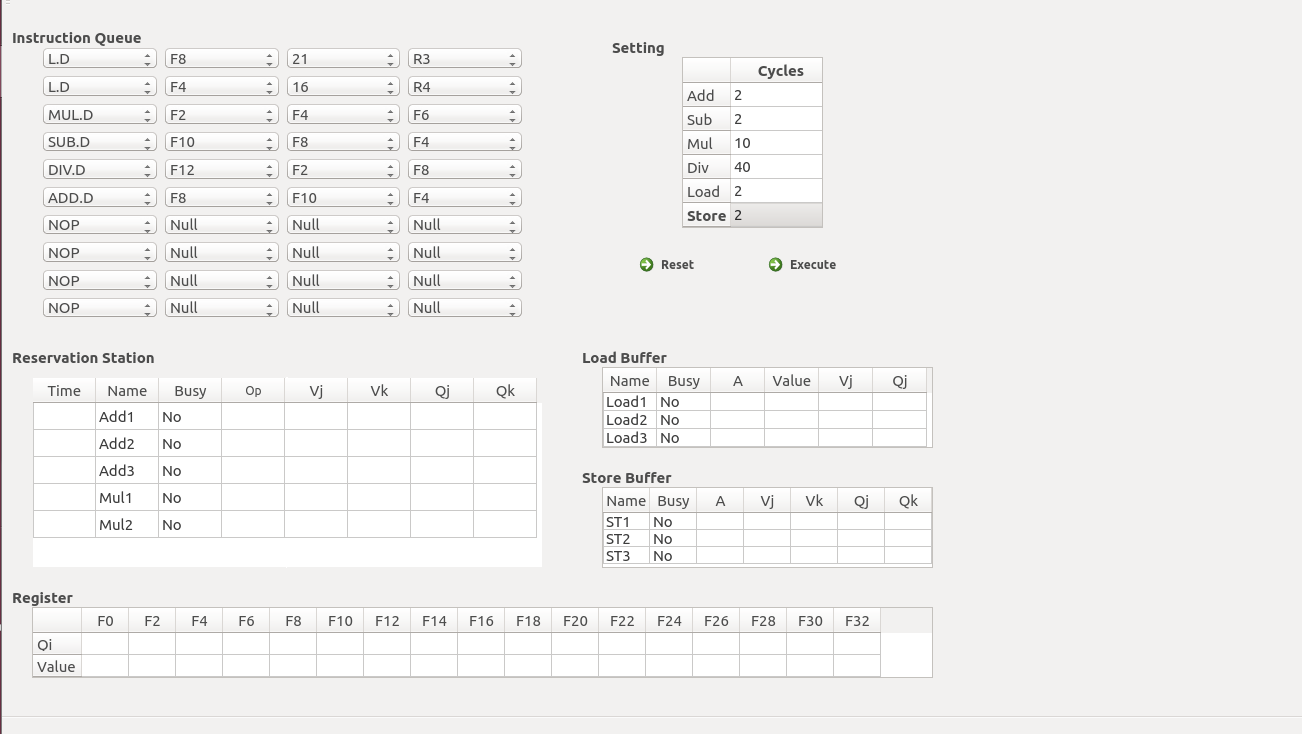
\includegraphics[width=.8\textwidth]{./frontend1.png}
%	\caption{参数设置}
	\end{center}
	
	\subsubsection*{执行指令}
	\begin{center}
	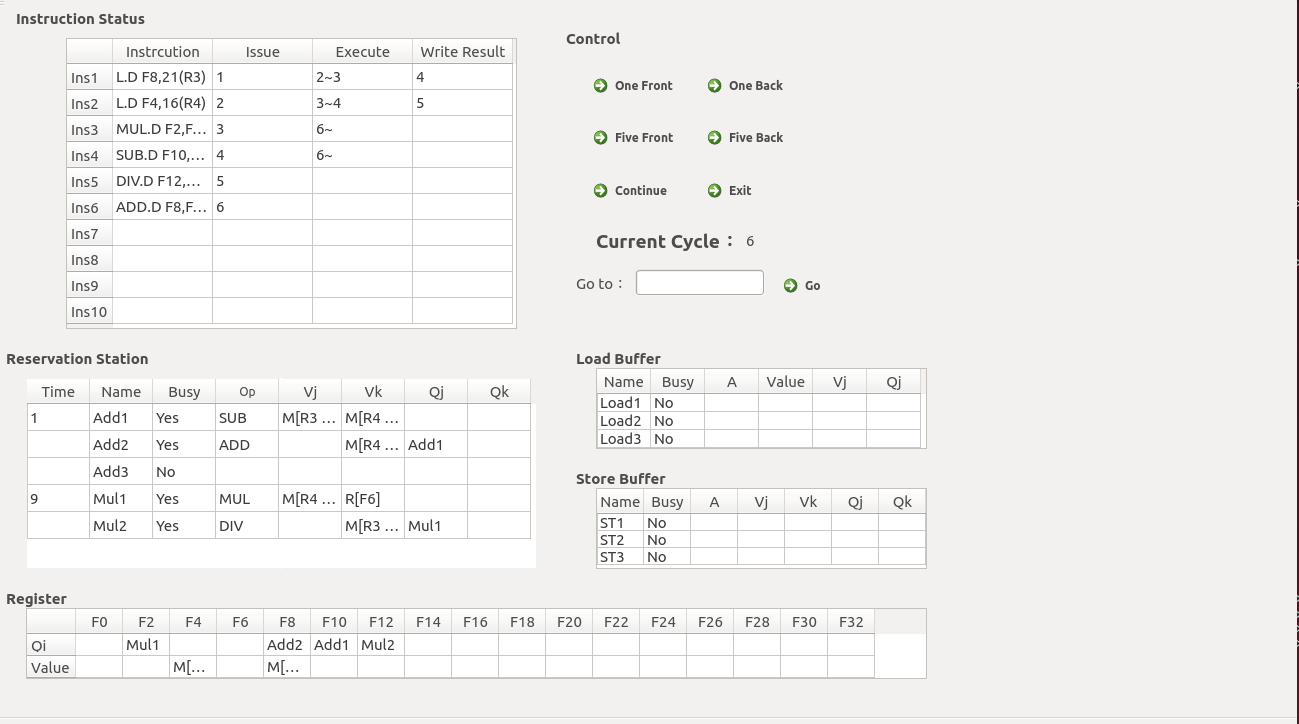
\includegraphics[width=.8\textwidth]{./frontend2.png}
	\end{center}
%	\caption{指令执行}
%	\end{figure}
	
	\subsection*{后端} \textit{cdb.h, virtualregister.h, tomasulo.h tomasulo.cpp}代码组成\textit{Tomasulo}算法的后端.后端主要负责\textit{Tomasulo}算法的具体实现. 其中\textit{virtualregister.h}中包含了所有实现\textit{Tomasulo}算法所需要的数据结构,如\textit{reservation station, register status, load buffer}等.\textit{tomasulo.cpp}是\textit{Tomasulo}算法的具体实现细节,包括指令的发射(\textit{issue()}),执行(\textit{execute()}),结果的写回(\textit{writeResult()})等函数的实现.另外cdb.h中实现了\textit{common data bus}结构,可以控制\textit{Tomasulo}算法中一个时钟周期内写结果的个数.

\section{问题解答}
	\subsection*{周期五保留站状态}
%	\begin{figure}[!htb]
	\begin{center}
		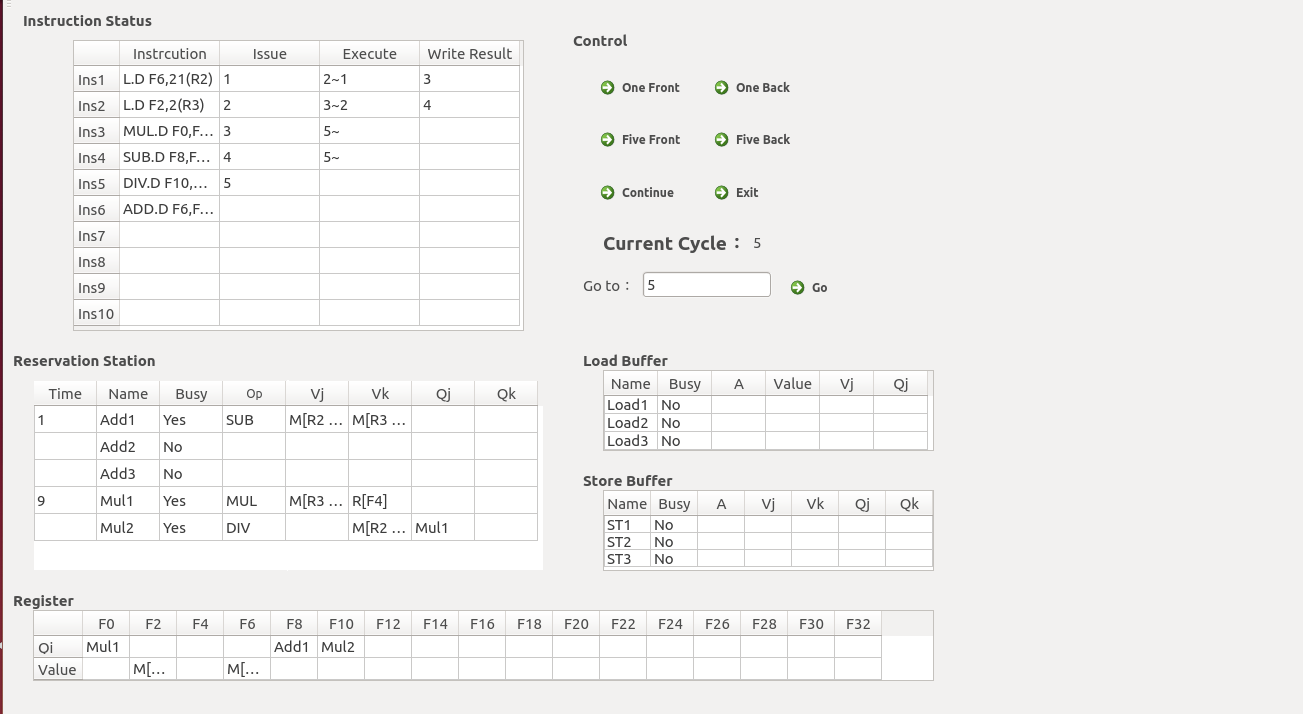
\includegraphics[width=.8\textwidth]{./cycle5.png}
	\end{center}
%	\caption{周期五}
%	\end{figure}
	\subsection*{周期十保留站等相关器件状态}
%	\begin{figure}[!htb]
	\begin{center}
		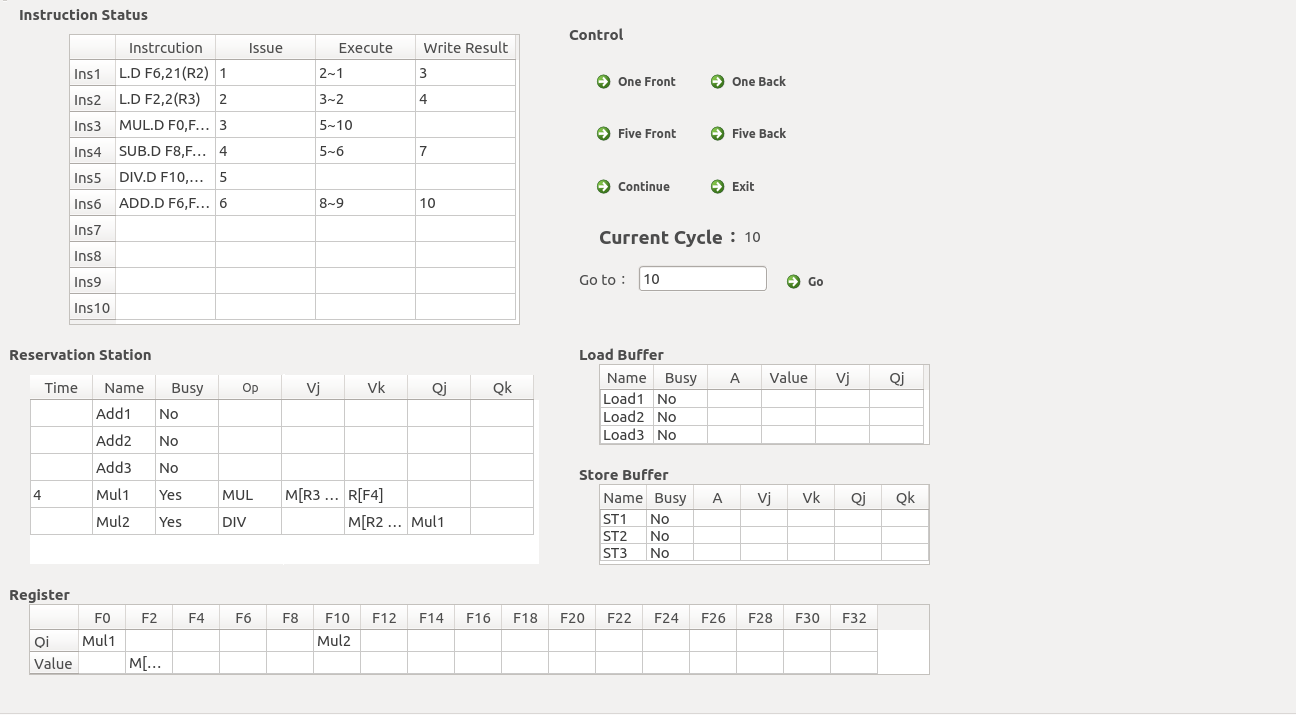
\includegraphics[width=.8\textwidth]{./cycle10.png}
	\end{center}
%	\caption{周期十}
%	\end{figure}
\section{总结}
	\paragraph{} 通过实现\textit{Tomasulo}算法,对该算法的具体细节有了更深入的掌握,同时对其提高指令级并行的原理和效果有了直观的了解和感受,对系统内部指令执行的具体细节有了更深入的理解和掌握.感受到提高指令并行能力对机器性能的影响.
\end{document}